\begin{figure}[h!]
    \centering
    \caption{Effects of \emph{Plan Cuadrante} on Trust and Police Effectiveness}
    \label{fig:effectiveness_es}
    \begin{subfigure}[t]{0.48\textwidth}
        \centering
        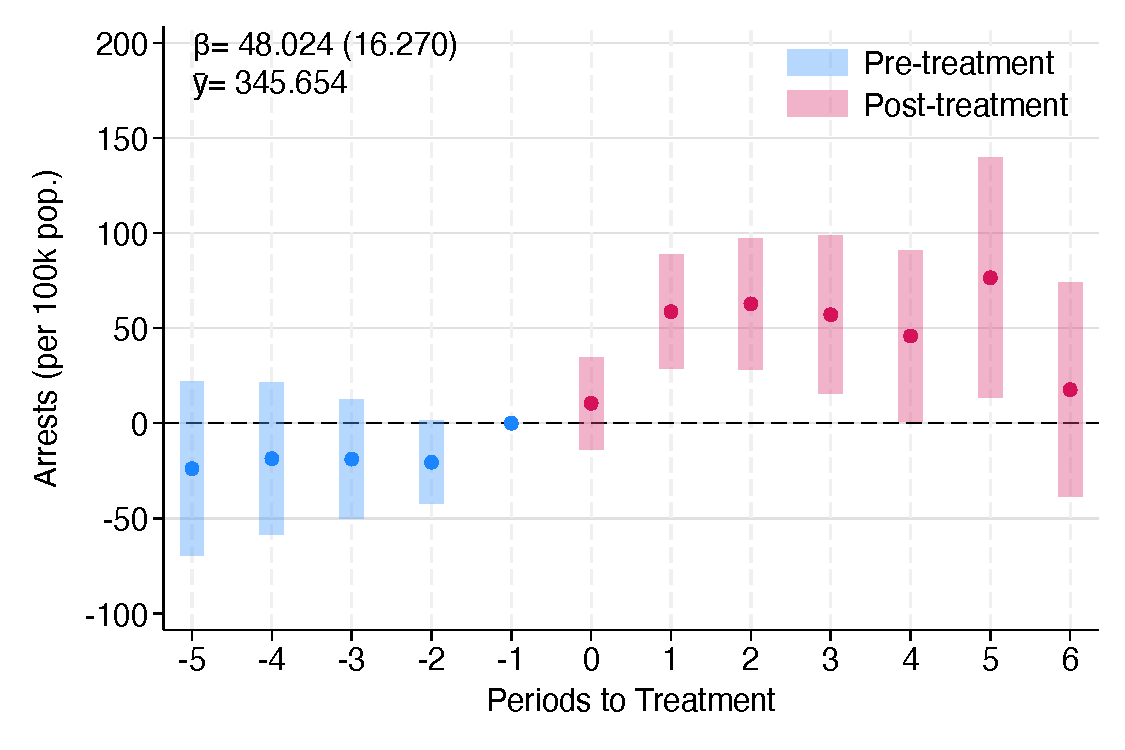
\includegraphics[width=\linewidth]{../manuscript/Graphs/totalarrestscrime_allcomunas.pdf}
        \caption{Arrests (per 100k pop.)}
    \end{subfigure}\hfill
    \begin{subfigure}[t]{0.48\textwidth}
        \centering
        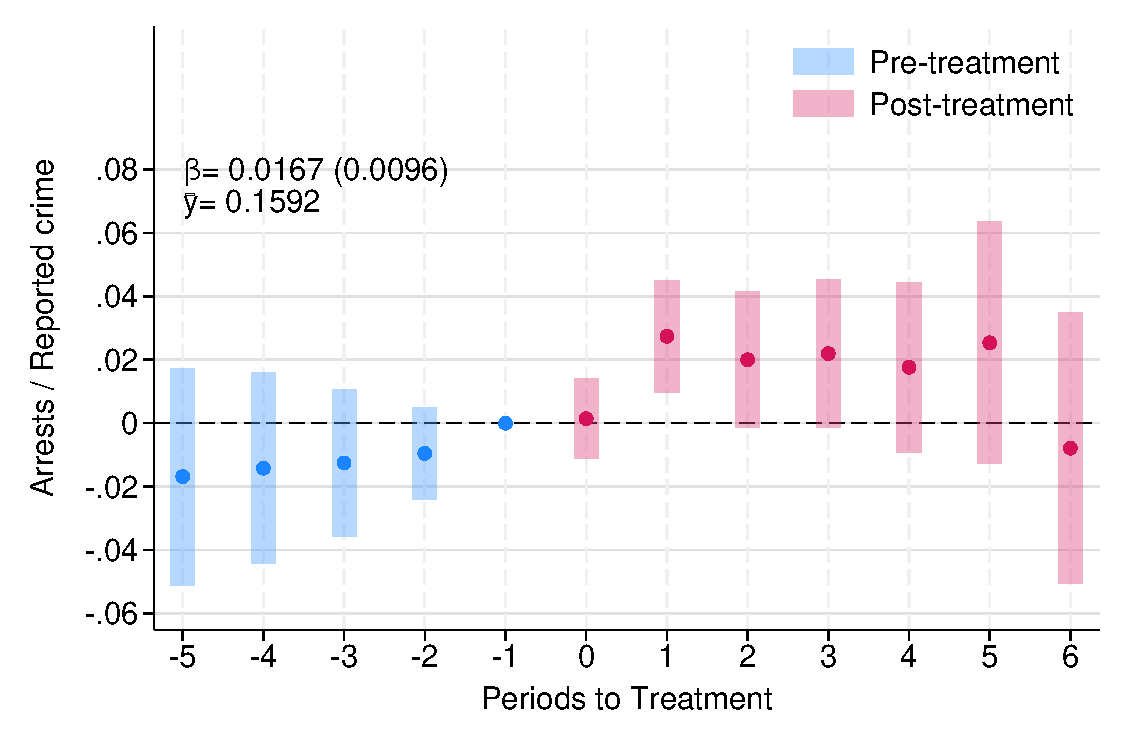
\includegraphics[width=\linewidth]{../manuscript/Graphs/arrests_over_reportedcrime_allcomunas.pdf}
        \caption{Arrests / Reported crime}
    \end{subfigure}
    \\[8pt]
    \begin{subfigure}[t]{0.48\textwidth}
        \centering
        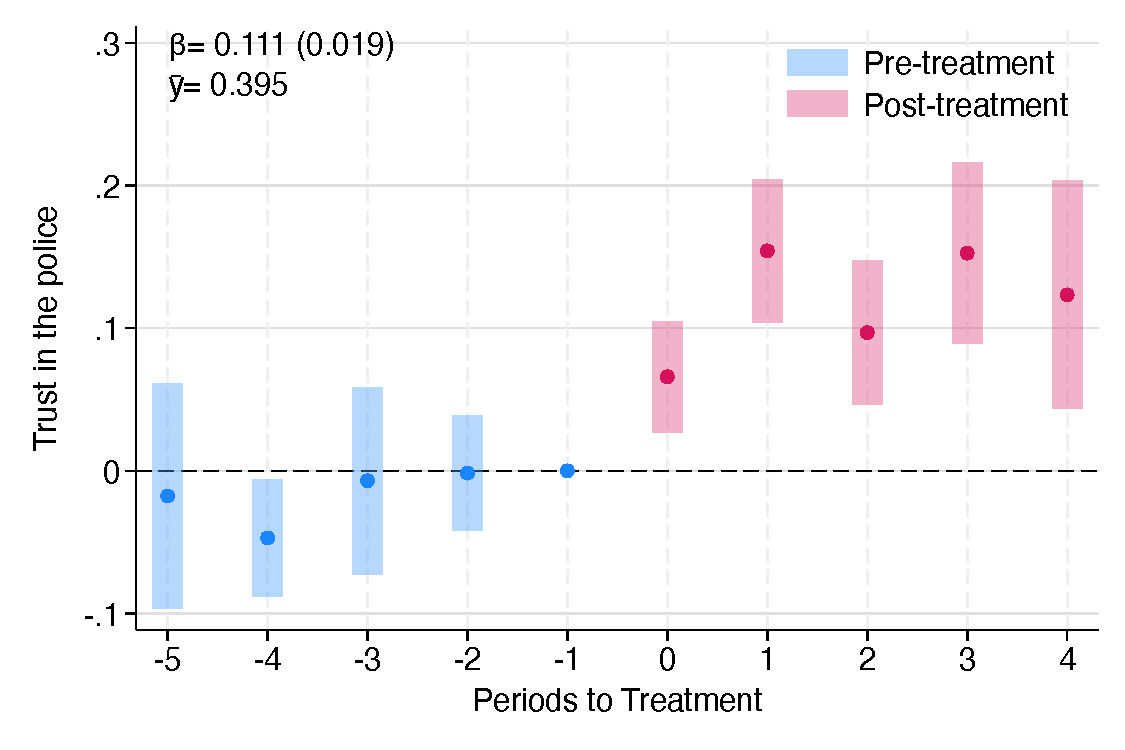
\includegraphics[width=\linewidth]{../manuscript/Graphs/results_trustcarabineros.pdf}
        \caption{Trust in the police}
    \end{subfigure}
    \\[10pt]
    \begin{minipage}{0.99\textwidth}
    \footnotesize Notes: This figure shows the dynamic effects of \emph{Plan Cuadrante} on measures of police effectiveness and trust in the police. The estimation is conducted using the procedure developed in \citet{Callaway} for difference-in-differences with staggered treatment adoption. The dots in the figure represent the estimated coefficients and the bars behind them 95\% confidence intervals. Standard errors are clustered at the municipality level using the wild bootstrapping procedure. The pooled effect and the mean outcome before the introduction of the treatment---computed as in Figure \ref{fig:figure02}, using only the pre-treatment observations of treated units---is also presented in each panel. Panel (a) reports the effect of \emph{Plan Cuadrante} on the number of arrests per 100,000 inhabitants using administrative data. Panel (b) reports the effect on the ratio of arrests to reported crime---the share of reported offenses that result in an arrest, a measure of police clearance or apprehension effectiveness---using administrative data. Panel (c) reports the effect on trust in the police using the ENUSC survey. Panel (a) includes 3,293 observations; panel (b), 3,263; and panel (c), 60,010 observations.
    \end{minipage}
\end{figure}
